\section{The iCub Humanoid Robot\label{sec:icub}}

\begin{figure}[tpb]
\centering
    \begin{subfigure}[b]{0.48\textwidth}
        \centering
        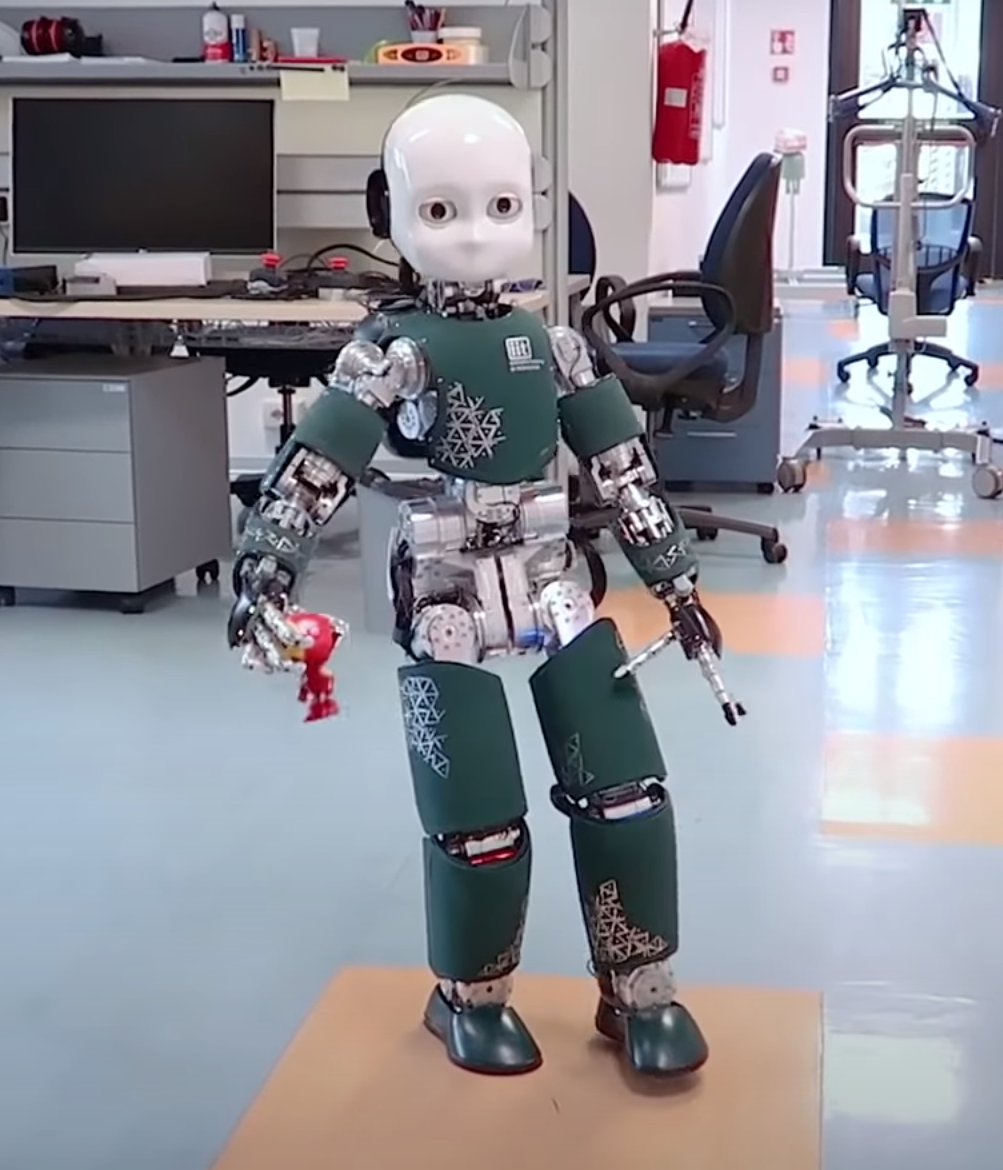
\includegraphics[width=\textwidth]{chapter_introduction/figures/iCubGenova04.png}
        \caption{The iCub v2.7 robot}
        \label{fig:iCubGenova04}
    \end{subfigure}
    \hfill
    \begin{subfigure}[b]{0.48\textwidth}
        \centering
        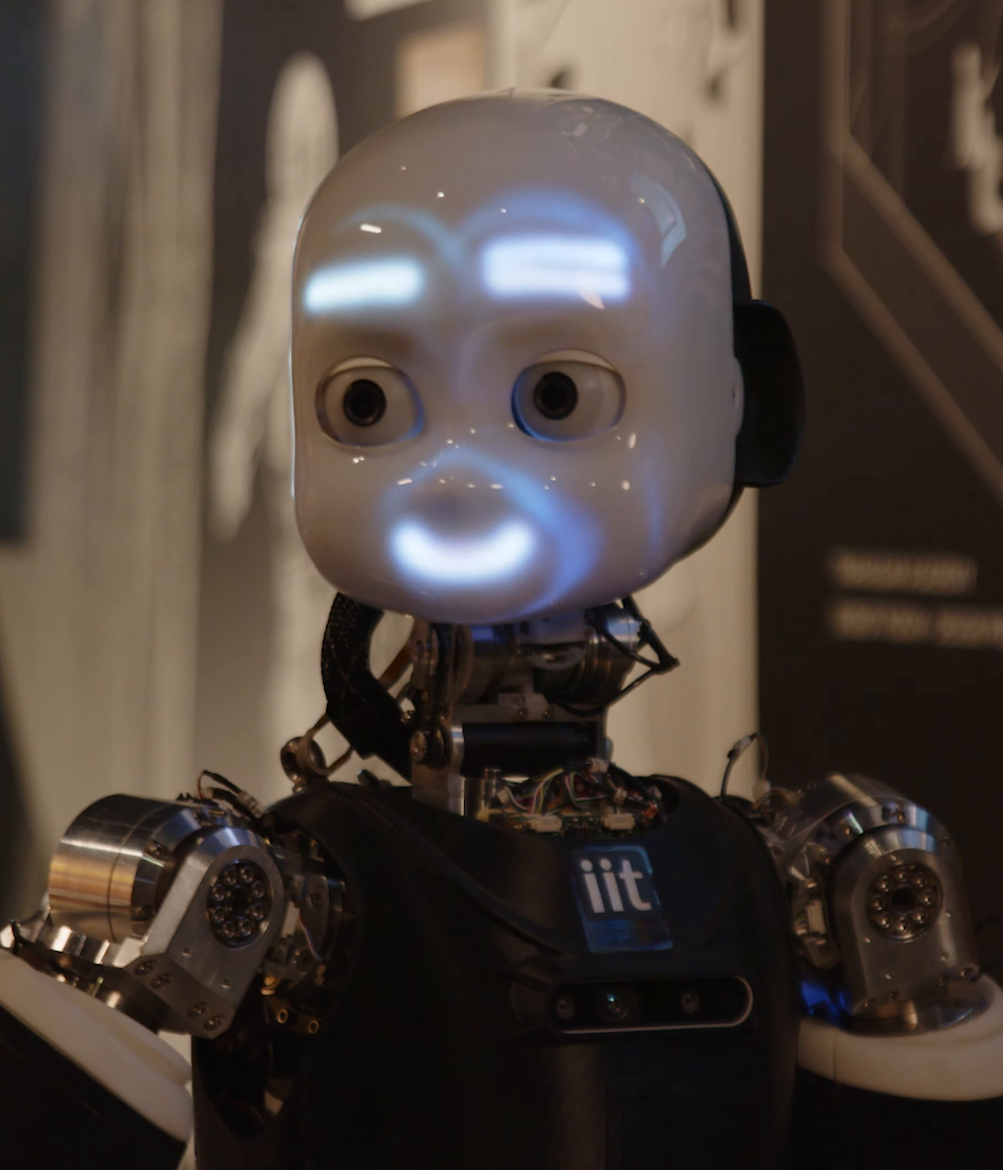
\includegraphics[width=\textwidth]{chapter_introduction/figures/iCubGenova09.png}
        \caption{The iCub v3 robot}
        \label{fig:iCubGenova09}
    \end{subfigure}
    \caption{The two versions of the iCub humanoid robot.}
	\label{fig:icub}
\end{figure}


\begin{figure}[tpb]
\centering
    \begin{subfigure}[b]{0.48\textwidth}
        \centering
        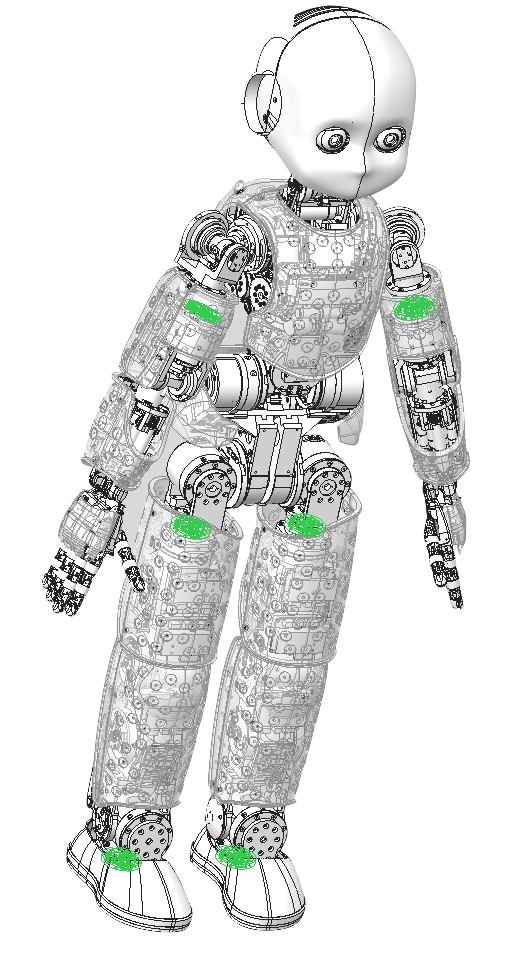
\includegraphics[height=\textwidth]{chapter_introduction/figures/icub_ft.png}
        \caption{Distribution of the six-axis force-torque}
        \label{fig:iCubGenova04_ft}
    \end{subfigure}
    \hfill
    \begin{subfigure}[b]{0.48\textwidth}
        \centering
        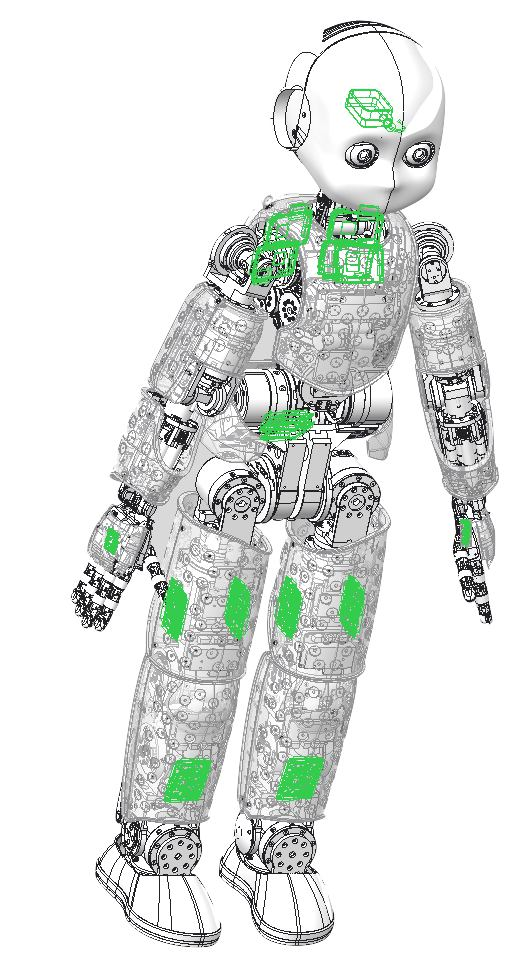
\includegraphics[height=\textwidth]{chapter_introduction/figures/icub_imu.png}
        \caption{Distribution of the inertial sensors}
        \label{fig:iCubGenova04_imu}
    \end{subfigure}
    \caption[FT and IMU distribution on iCub v2.7]{Distribution of the six embedded six-axis force-torque sensors (a) and of the inertial sensors (b) on iCub v2.7.}
	\label{fig:iCubGenova04_sensors}
\end{figure}

The iCub Humanoid Robot is an open source state-of-the-art robotic platform created as part of the European project RobotCub~\citep{Tsagarakis2007,Natale2017,Parmiggiani2012,Metta2010} at the Italian Institute of Technology.
The iCub has been regularly updated with upgrades and new features since its first release in 2006. More than 40 partnering institutions in Europe, Asia, and the United States have received copies of iCub. 

Because innovations are constantly issued and integrated into the many iCubs, all robot copies have distinct features based on their release date, the maintenance upgrades conducted over the years, and the individual customization of each iCub. The algorithms discussed in the thesis have been tested on two versions of the iCub robots, namely iCub v2.7 and iCub v3. Section~\ref{sec:icub2.7} presents the characteristics of iCub v2.7, while Section~\ref{sec:iCub3} introduces iCub v3. 

\subsection{The iCub v2.7 robot\label{sec:icub2.7}}

Figure~\ref{fig:iCubGenova04} depicts the iCub humanoid robot v2.7, which is $\SI{104}{\centi\meter}$ tall and weighs $\SI{33}{\kilo\gram}$. It has 54 degrees of freedom in total, including those in the hands and eyes. Only 23 joints are used for locomotion and are distributed as follows: 4 joints in the arm, 3 of which in the shoulder and one in the elbow, 3 joints in the torso, and 6 joints in each leg. 
The torso and shoulder joints are mechanically coupled and driven by tendon mechanisms. All 23 joints are powered by brushless electric motors equipped with Harmonic Drive transmissions with a reduction ratio of 1/100.

A series of electronic boards known as 2FOC, EMS, and MC4Plus operate the iCub motors. The 2FOC boards use an incremental optical encoder positioned on the motor shaft to regulate the magnetic flux of a brushless motor by setting a reference PWM (Pulse Width Modulation). The EMS boards, on the other hand, are linked to the 2FOC boards and implement three control strategies, namely position, velocity, and torque control. The electronic boards are connected through an Ethernet network in daisy chain.
\par
A three-degree-of-freedom accelerometer and three-degree-of-freedom gyroscopes are included on each motor control board. In addition, the robot's head is equipped with a full-fledged Inertial Measurement Unit, which includes a 3 DOF magnetometer, accelerometer, and gyroscope. Figure~\ref{fig:iCubGenova04_imu} shows how these designs offer the iCub v2.7 with a large amount of distributed inertial sensing, which has been exploited for precise calibration in~\citep{Guedelha2016Self-calibrationMeasurements}.
\par
Differently from other state-of-the-art robots \citep{Englsberger2015OverviewTORO,Stasse2017TALOS:Applications}, the iCub humanoid robot v2.7 does not mount pure torque sensors on the joints. As a consequence, the internal joint torques cannot be directly measured. However the robot is equipped with 6 inertial six-axis force-torque sensors - Figure~\ref{fig:iCubGenova04_ft}. Four of them are attached to the base of each limb, while two are mounted on the robot's ankles. The location of these sensors enables the estimation of internal joint torques and external force-torque, as described in~\citep{Fumagalli2012} for a single limb and in \citep[Chapter~4]{Traversaro2017ModellingDynamics} for the whole-body case.
\par
Finally, the robot head is equipped with a 4$^{\text{th}}$ generation Intel\textsuperscript{\textregistered} Core i7@1.7GHz and 8GB of RAM running Ubuntu Linux. Finally, the connection to the robot can be established through an Ethernet cable or thought a standard 5GHz Wi-Fi network.

\begin{figure}[t]
\centering
    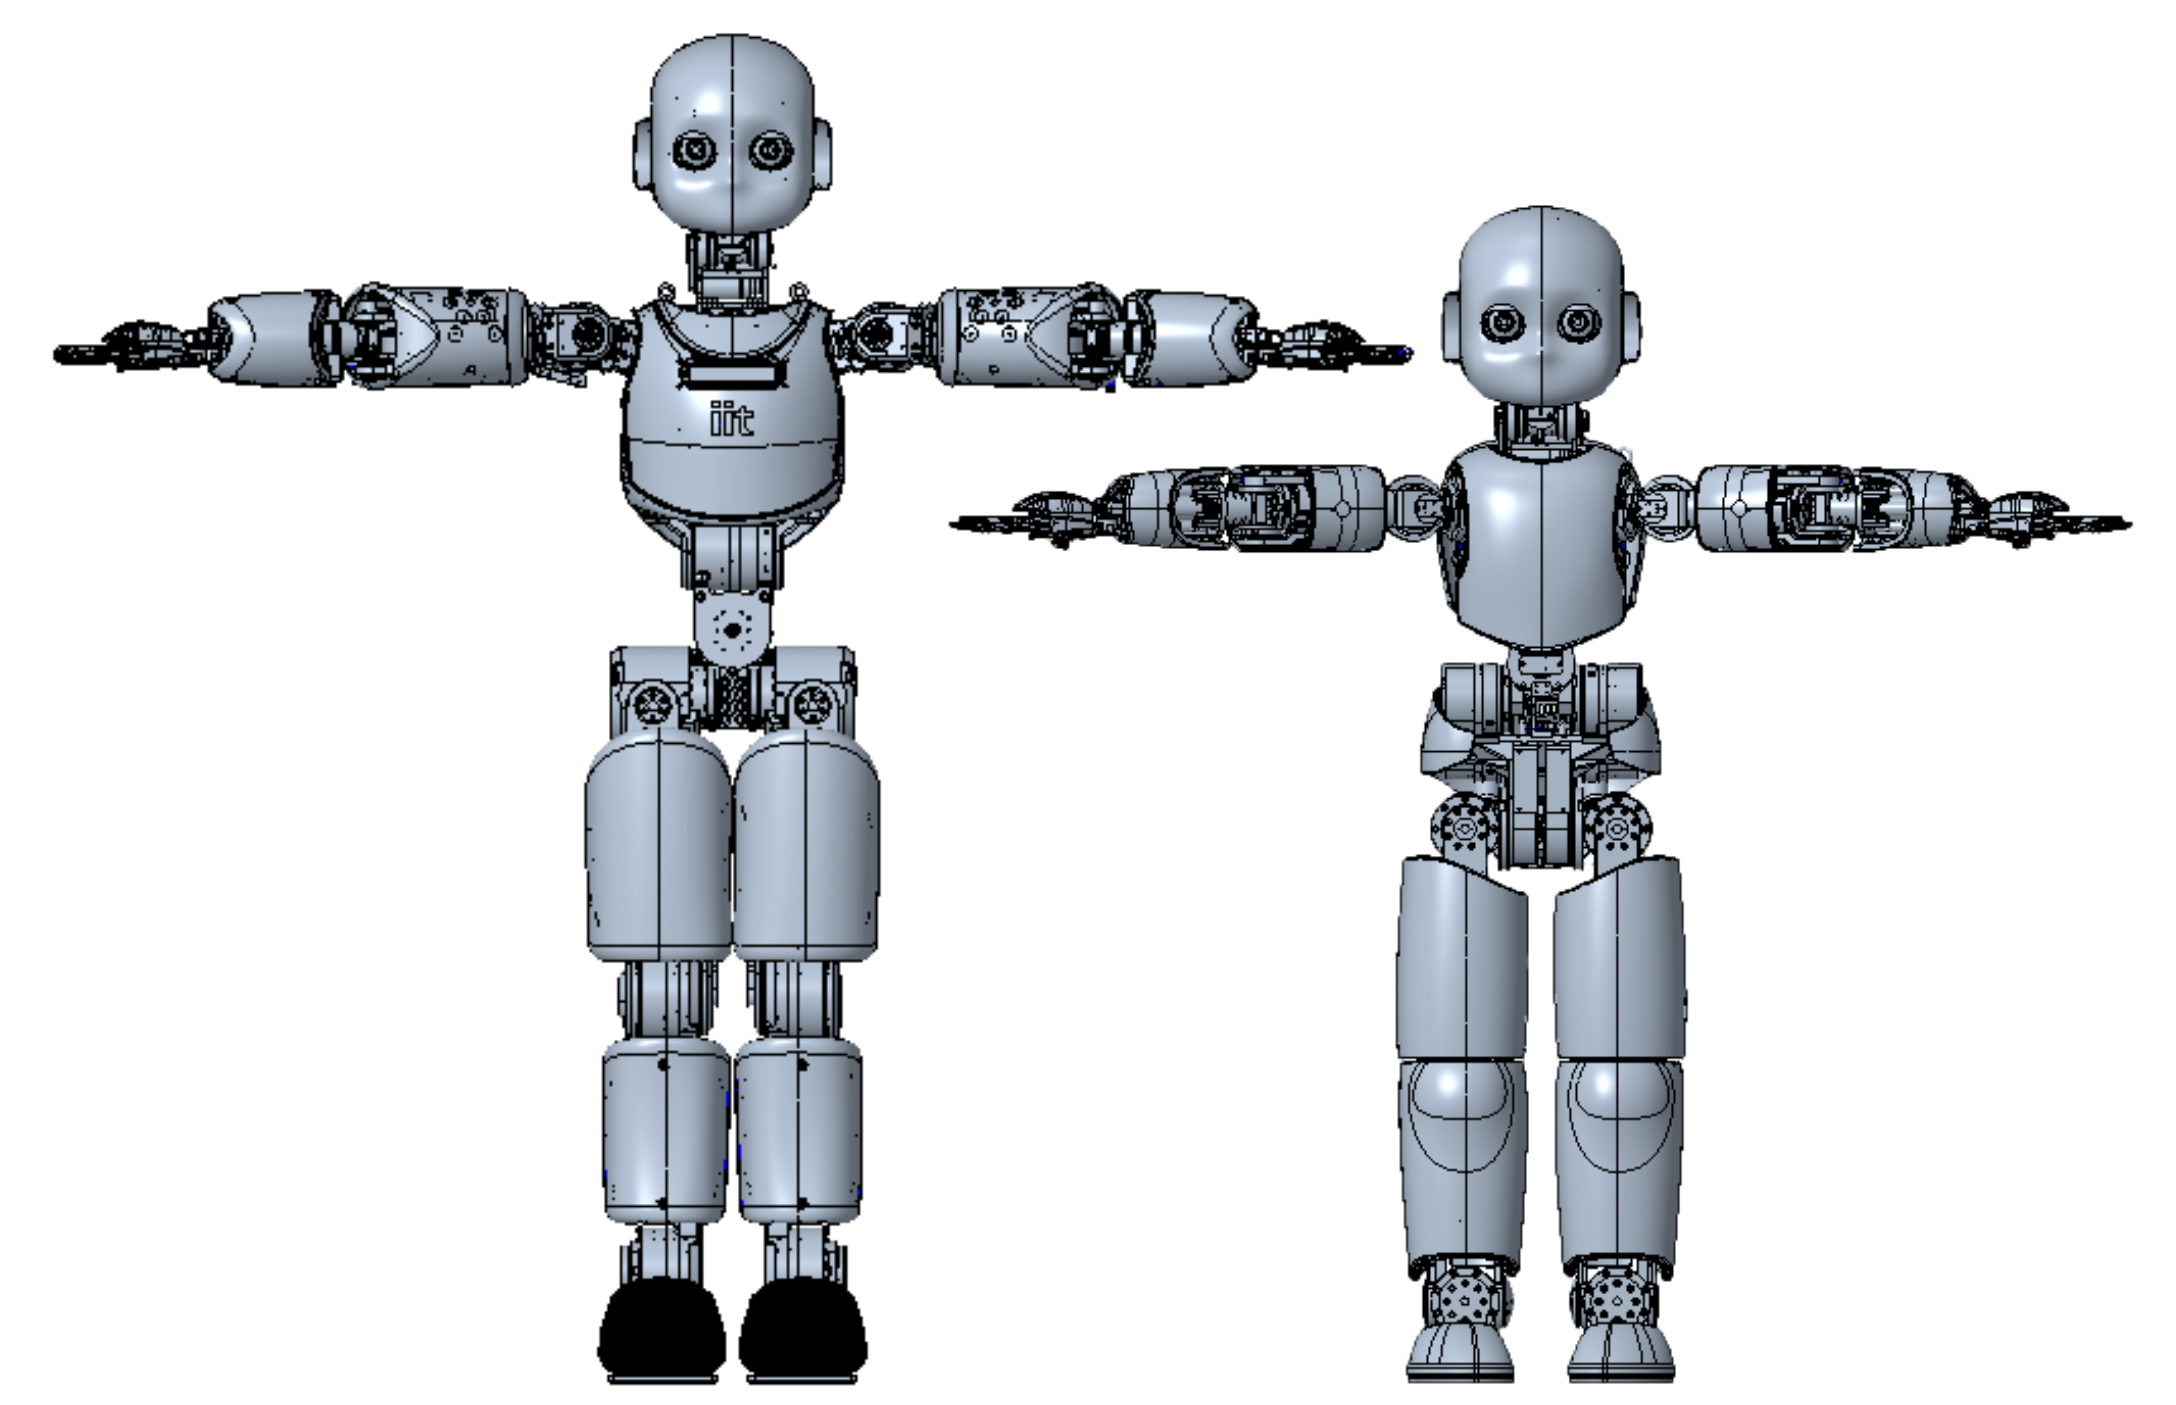
\includegraphics[width=\textwidth]{chapter_introduction/figures/icub_comparison.png}
    \caption{The iCub3 robot side to side to the classical iCub v2.7.
    \label{fig:icub_comparison}}
\end{figure}


\subsection{The iCub v3 robot} \label{sec:iCub3}
The iCub v3 humanoid robot, depicted in Figure \ref{fig:iCubGenova09}, is a state-of-the-art robotic platform developed at the Italian Institute of Technology and can be seen as an evolution of the iCub v2.7 presented in Section~\ref{sec:icub2.7}. 
\par
The iCub v3 humanoid robot is larger than a traditional iCub v2.7 platform, standing $\SI{25}{\centi\meter}$ higher and weighing $\SI{22}{\kilo\gram}$ heavier. The robot is $\SI{125}{\centi\meter}$ tall and weighs $\SI{52}{\kilo\gram}$. Figure \ref{fig:icub_comparison} shows the different dimensions of the two platforms.
The greater weight necessitates more powerful leg motors. As a consequence of the increased size of the actuators, a new approach to the knee and ankle pitch joints was necessary. Specifically, instead of being on the same axis, the motor and actuator are separated and linked by belts. Similarly to iCub v2.7, the iCub v3 robot possesses in total 54 degrees of freedom, including those in the hands and the eyes, and only 23 joints are used for locomotion. However, unlike iCub v2.7, the torso and shoulder joints are not tendon-driven. In fact, the joints are directly connected to the motor shaft throughout the serial direct mechanisms. This provides for a larger range of motion and mechanical toughness.
All 23 joints used for locomotion are powered by brushless three-phase electric motors equipped with Harmonic Drive transmissions. 
Each foot is made up of two rectangular parts, each measuring $\SI{25}{\centi\meter}$ in length and $\SI{10}{\centi\meter}$ in width.
\par
Similarly to iCub v2.7, iCub v3 is equipped with a vast array of sensors, including accelerometers, gyroscopes, and force/torque sensors. Six six-axis force/torque (F/T) sensors are included in the iCub. Two are placed on each shoulder and two are attached to each foot, linking the two portions of the feet to the ankle assembly. The readouts of the F / T sensors are used to estimate the internal joint torques and the external force-torque, as presented in \citep[Chapter~4]{Traversaro2017ModellingDynamics}.

\subsection{Software infrastructure}
A computer infrastructure is required to control the robot. To
this end, the Yet Another Robot Platform (YARP) middleware~\citep{Metta2006} is exploited. YARP is an open-source multi-platform middleware whose main purpose is to allow communication between the applications (modules), which can run on different computers. More specifically, YARP is a set of libraries, protocols, and tools to keep modules and devices cleanly decoupled. Indeed, it provides an abstraction layer to interact with physical devices, such as joint encoders and F/T sensors, independently of their actual implementation. Moreover, sensor acquisition and motor controllers are provided through YARP interfaces.
\par
Along with the YARP middleware, we took advantage of the iDynTree library~\citep{Nori2015} to design the controllers. iDynTree is a library of robot dynamics algorithms for control, estimation, and simulation. It is specifically designed for free-floating robots, but it is also possible to use it with fixed-base robots. It is written in \texttt{C++}, with Python and MATLAB interfaces. iDynTree contains support for reading and writing \texttt{URDF} files, making it possible to use it with any type of robot described by an \texttt{URDF}.
\par
Rapid prototyping is achieved thanks to iDyntree interfaces, which can be easily integrated into off-the-shelf Python libraries and Simulink and MATLAB toolbox. Controller prototyping also takes advantage of the Gazebo simulation environment \citep{Koenig04}. Gazebo is an open source simulator that can efficiently simulate complex multibody systems. The interface between the controller algorithms and the simulated version of the robot is handled through the corresponding YARP plugins \citep{MingoHoffman2014}. The plugins make the algorithm implementation transparent. In fact, they allow testing of the very same software on both the simulator and the real robot.